% https://tex.stackexchange.com/questions/311132/how-to-style-hrefs-underlined-and-coloured-throughout-the-document
\usepackage{xcolor,soul}
\usepackage{hyperref}
\hypersetup{colorlinks,urlcolor=blue}
\urlstyle{sf}

\makeatletter
\patchcmd{\hyper@link@}
{{\Hy@tempb}{#4}}
{{\Hy@tempb}{\ul{#4}}}
{}{}
\makeatother

\usepackage{pdfcomment}

%% ------------------------------------------------------------------------------
%% Headers and footers
\lhead{DRAFT -- Non-citable working paper}
% \lhead{}
% \rhead{}
\rfoot{DRAFT - DO NOT CITE}
%% ------------------------------------------------------------------------------

\fancypagestyle{nofooter}{%
\fancyfoot{}%
}

\begin{document}

\thispagestyle{empty}

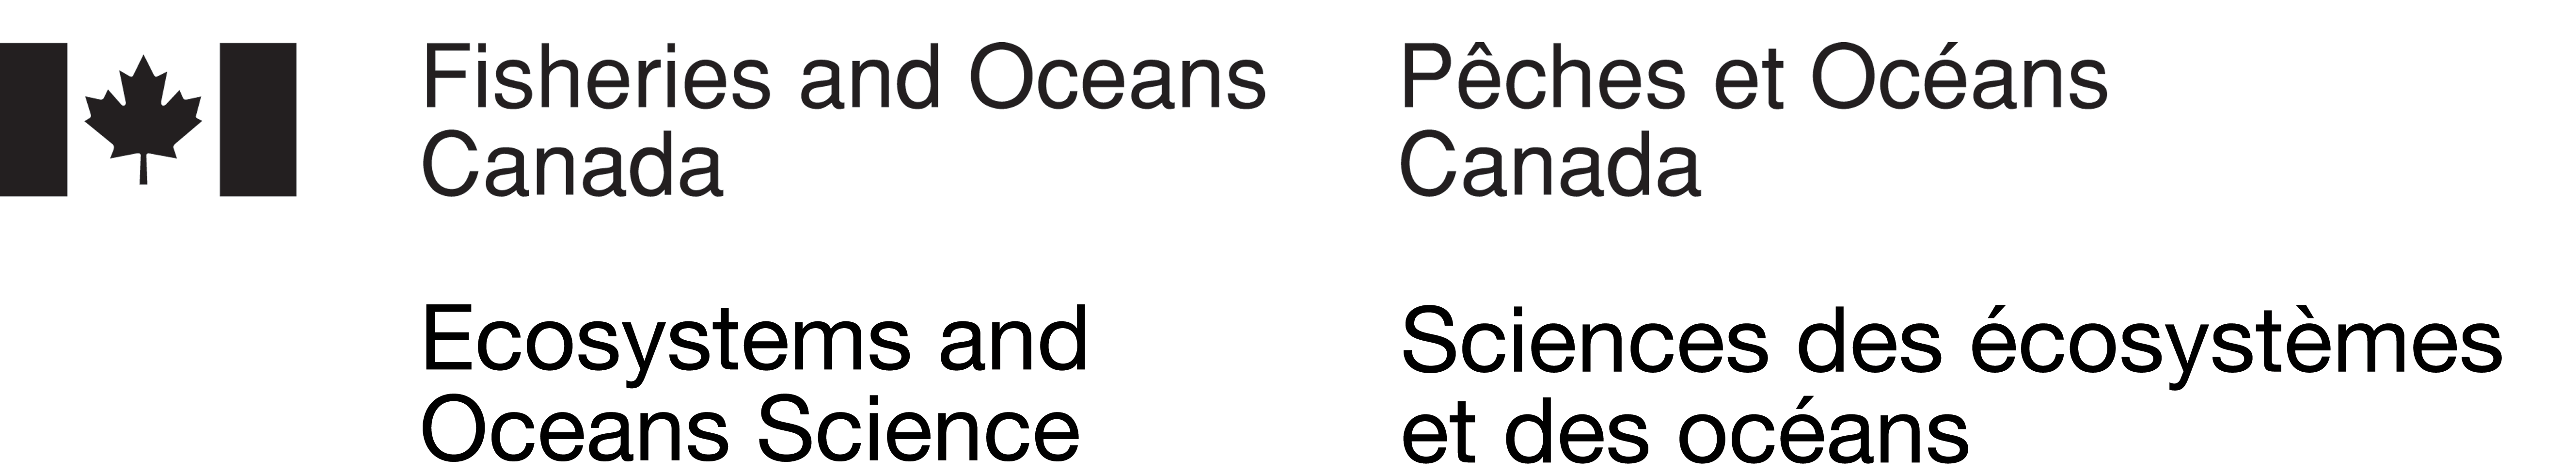
\includegraphics[width=9.14cm]{title-page-images/title-header.png}

\textbf{Canadian Science Advisory Secretariat (CSAS)}
\vspace{0.5mm}

\hrule

\vspace{-1.5mm}

\textbf{Research Document 2017/nnn}\\

\vspace{0.2cm}

\textbf{Pacific Region}

\vspace*{\fill}
\begin{center}

  \textbf{A reproducible data synopsis for British Columbia groundfish fisheries}

\vspace{.35cm}

Sean C. Anderson\textsuperscript{1}, First M. Last\textsuperscript{1} and First M. Last\textsuperscript{1}

\vspace{.35cm}

\textsuperscript{1}Pacific Biological Station, Science Branch,\\
Fisheries and Oceans Canada, 3190 Hammond Bay Road,\\
Nanaimo, British Columbia, V9T 6N7, Canada. 

\end{center}
\vspace*{\fill}

\hrule

\vspace{-4.0mm}
\parbox{9cm}{Release date (Month Year)}%
\begin{minipage}[t]{7.48cm}
\flushright

\includegraphics[width=3.54cm]{title-page-images/title-footer.png}%
\end{minipage}


\clearpage

\vspace*{\fill}

\begin{center}
\textbf{Foreword}
\end{center}
\vspace{-1.5mm}

This series documents the scientific basis for the evaluation of aquatic resources and
ecosystems in Canada. As such, it addresses the issues of the day in the time frames required
and the documents it contains are not intended as definitive statements on the subjects
addressed but rather as progress reports on ongoing investigations.

Research documents are produced in the official language in which they are provided to the Secretariat.

\vspace{1.5mm}

\begin{center}
\textbf{Published by:\\}
\vspace{0.2cm}
Fisheries and Oceans Canada\\
Canadian Science Advisory Secretariat\\
200 Kent Street\\
Ottawa ON K1A 0E6\\
\vspace{0.17cm}

\href{http://www.dfo-mpo.gc.ca/csas-sccs/}{http://www.dfo-mpo.gc.ca/csas-sccs/}\\
\href{mailto://csas-sccs@dfo-mpo.gc.ca}{csas-sccs@dfo-mpo.gc.ca}

\vspace{-3mm}

\includegraphics[scale=0.96]{title-page-images/recycle.png}

\vspace{-3mm}
\textcopyright\ Her Majesty the Queen in Right of Canada, 2017\\
ISSN 1919-5044
\end{center}

\vspace{-3mm}

\textbf{Correct citation for this publication:}\\
\vspace{0.2cm}
\hangindent=0.6cm Jones, S., Burns, E. and Smith, K. 2017. 
Title --- must be exactly as it appears on the cover page. 
DFO Can.\ Sci.\ Advis.\ Sec.\ Res.\ Doc. 2016/nnn. vi + xx p.
\vspace*{\fill}

\thispagestyle{nofooter}

